\documentclass[12pt]{book}
\usepackage[utf8]{inputenc}
\usepackage[T1]{fontenc}
\usepackage{tocbibind}
\usepackage{mathptmx}
\usepackage{geometry}
\usepackage{mathtools}
\usepackage[english]{babel}
\usepackage{graphicx}
\usepackage{subcaption}
\usepackage{stackengine}
\usepackage[os=win]{menukeys}
\usepackage{hyperref}
\usepackage{xcolor}
\usepackage{tikz}
\usepackage[yyyymmdd,hhmmss]{datetime}
\usepackage{etoolbox}
\usepackage[inline]{enumitem}
\usepackage{listings}
\usepackage{booktabs}

\newcommand{\WindowsLogo}{\raisebox{-0.1em}{
\includegraphics[height=0.8em]{images/logo/Windows_3_logo_simplified}}}
%\newcommand{\PowerLogo}{\raisebox{-0.1em}{
\includegraphics[height=0.8em]{images/logo/power}}}
\newcommand{\WinKey}{\keys{\WindowsLogo}}
\newcommand{\PowerKey}{\keys{\PowerLogo}}

%%%%% Mengganti label "Contents" ke "Daftar Isi" %%%%%
\addto\captionsenglish{\renewcommand{\contentsname}{Daftar Isi}}

%%%%% Mengganti label "Chapter" ke "Bab" %%%%%
\addto\captionsenglish{\renewcommand{\chaptername}{Bab}}

%%%%% Mengganti label "Figure" ke "Gambar" %%%%%
\addto\captionsenglish{\renewcommand{\figurename}{Gambar}}

%%%%% Mengganti label "List of Figures" ke "Daftar Gambar" %%%%%
\addto\captionsenglish{\renewcommand{\listfigurename}{Daftar Gambar}}

%%%%% Mengganti label "Table" ke "Tabel" %%%%%
\addto\captionsenglish{\renewcommand{\tablename}{Tabel}}

%%%%% Mengganti label "List of Tables" ke "Daftar Table" %%%%%
\addto\captionsenglish{\renewcommand{\listtablename}{Daftar Tabel}}

\hypersetup{
	colorlinks=true, %set true if you want colored links
	linktoc=all,     %set to all if you want both sections and subsections linked
	linkcolor=blue,  %choose some color if you want links to stand out
	urlcolor=blue,   %url color
}

\geometry{
	a4paper,
	left=10mm,
	right=10mm,
	top=15mm,
	bottom=15mm,
}

\date{}

\hypersetup{citecolor=black}

\definecolor{LightGray}{gray}{0.95}

%\pagecolor[rgb]{0.1,0.1,0.1}
%\color[rgb]{1,1,1}

\lstset
{
	language=bash,
	breaklines=true,
	basicstyle=\tt\normalsize,
	frame = single
}

\begin{document}

	\frontmatter
	\begin{titlepage}
		\centering
		{\LARGE \bf Panduan Dasar Draft PCB Menggunakan KiCAD}
		\vfill
		{\Large Achmadi ST MT}
		\vfill
		
\includegraphics[width=250pt]{images/logo/logoviblab}
		\vfill
		\vfill
	\end{titlepage}

	%%%%%%%%%%%%%%%%%%%%%%%%%%%%%%%%%%%%%%%%%%%%%%%%%%%%%%%%%%%%%%%%%

	\newpage
	\tableofcontents
	\listoffigures
	\listoftables

	%%%%%%%%%%%%%%%%%%%%%%%%%%%%%%%%%%%%%%%%%%%%%%%%%%%%%%%%%%%%%%%%%

	%%%%%%%%%%%%%%%%%%%%%%%%%%%%%%%%%%%%%%%%%%%%%%%%%%%%%%%%%%%%%%%%%

	\newpage
	\chapter{Penggunaan Buku}

	\section{Umum}
	Buku ini dibuat dengan tujuan penggunaan utama sebagai panduan digital untuk mempermudah search dan copy-paste.
	Anda tidak perlu mencetak buku ini ke bentuk kertas.
	Seluruh navigasi buku ini diharapkan menggunakan klik ke hyperlink di Daftar Isi,
	atau menggunakan tampilan \textbf{Index} yang tersedia di \textbf{SideBar} program pembaca PDF yang anda gunakan.

	\section{Petunjuk}
	Beberapa petunjuk yang digunakan di buku ini:
	\begin{itemize}
		\item \textbf{Cetak Tebal}: Menginformasikan identifier (keyword, variabel, fungsi, alamat, nama file, dst) yang berada di suatu paragraf
		\item \textit{Cetak Miring}: Bersama simbol panah (->) dan simbol lain, menginformasikan langkah-langkah klik menu/tombol.
		\item \textbf{TIPS:} Menginformasikan hal-hal yang dapat membantu atau pengetahuan tambahan.
		\item \textbf{PERINGATAN:} Menginformasikan hal-hal yang bener-benar harus diperhatikan.
	\end{itemize}

	%%%%%%%%%%%%%%%%%%%%%%%%%%%%%%%%%%%%%%%%%%%%%%%%%%%%%%%%%%%%%%%%%

	\newpage
	\mainmatter
	\chapter{Program KiCAD}

	\section{Pengenalan}

	KiCAD adalah paket software EDA (Electronic Design Automation) yang dikembangkan untuk perancangan papan sirkuit elektronik tercetak (Printed Circuit Board atau PCB)
	secara professional yang bersifat gratis dan terbuka.

	KiCAD dapat disandingkan dengan perangkat perancangan PCB professional lain seperti Altium, Diptrace, EasyEDA, dan lainnya.
	KiCAD tersedia untuk sistem operasi Windows, GNU/Linux, dan MacOS.\\

	Berikut adalah tampilan 4 software utama dalam paket software KiCAD:
	\begin{figure}[!ht]
		\centering
		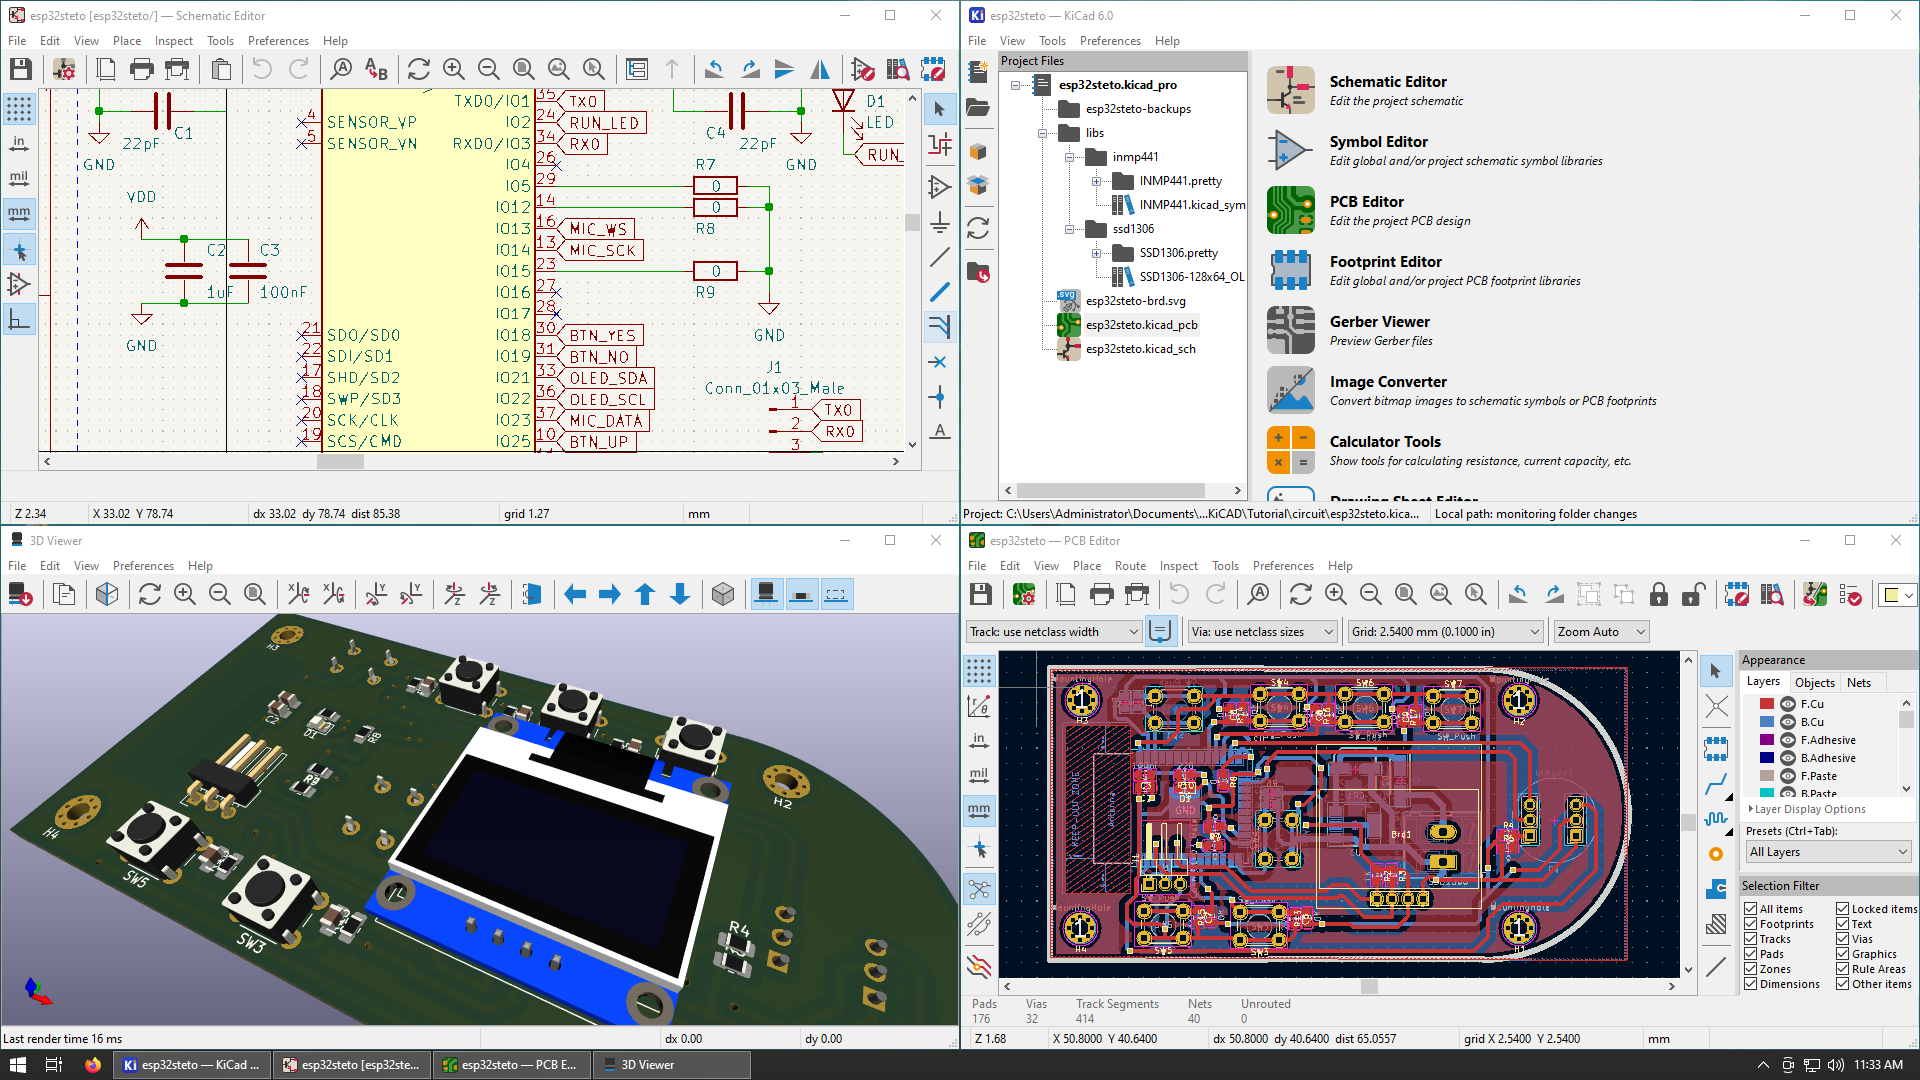
\includegraphics[width=\textwidth]{images/kicad_windows10}
		\caption{Tampilan KiCAD Windows 10}
	\end{figure}

	\textbf{TIPS:} Sepanjang tutorial, akan digunakan tampilan Windows 10 atau GNU/Linux sebagai acuan.
	Namun tutorial yang sama akan dapat pula digunakan di sistem operasi lain seperti Windows 8 dan Windows 11.\\

	\textbf{PERINGATAN:} Versi KiCAD yang akan digunakan adalah versi 6, dimana untuk sistem operasi Windows
	hanya bisa diinstal di Windows 8 dan selanjutnya.
	Untuk pengguna Windows 7 dan sebelumnya, disarankan menggunakan KiCAD versi 5.

	\newpage
	\section{Instalasi}

	\subsection{GNU/Linux}

	Berikut panduan instalasi KiCAD untuk dua jenis GNU/Linux yang populer, yaitu:
	\begin{itemize}
		\item Arch based, seperti Arch-Linux dan Manjaro.
		\item Ubuntu based, seperti Ubuntu-Mate dan Xubuntu.
	\end{itemize}

	\textbf{TIPS:} Untuk sistem operasi GNU/Linux, semua instalasi dilakukan via perintah di
	terminal emulator dengan sumber paket instalasi adalah mirror terdekat dari repository server masing-masing sistem operasi.\\

	\textbf{TIPS:} Perlu diingat untuk instalasi di GNU/Linux dibutuhkan hak akses administratif (umumnya sudo),
	sehingga dibutuhkan password akses tersebut.

	\subsubsection{Arch based}

	Untuk instalasi software KiCAD dan pustaka dasar, perintahnya adalah:

	\begin{lstlisting}
sudo pacman -S kicad kicad-library
	\end{lstlisting}

	Ukuran download berkisar 70MB dan ukuran instalasi berkisar 400MB.\\

	Kemudian untuk instalasi pustaka model komponen 3D, perintahnya adalah:

	\begin{lstlisting}
sudo pacman -S kicad-library-3d
	\end{lstlisting}

	Ukuran download berkisar 350Mb dan ukuran instalasi berkisar 5GB.\\

	\textbf{TIPS:} Jika diperlukan, lakukan update/upgrade sistem operasi dengan perintah:

	\begin{lstlisting}
sudo pacman -Syu --noconfirm
	\end{lstlisting}

	\subsubsection{Ubuntu based}

	Untuk instalasi KiCAD pada sistem operasi ini, digunakan sumber PPA khusus KiCAD 6:\\
	\url{https://launchpad.net/~kicad/+archive/ubuntu/kicad-6.0-releases} \\

	Pertama, tambahkan repository tersebut dengan perintah:
	\begin{lstlisting}
sudo add-apt-repository ppa:kicad/kicad-6.0-releases
sudo apt update
	\end{lstlisting}

	Kemudian perintah untuk instalasi seluruh paket lengkap (termasuk pustaka komponen 3D):
	\begin{lstlisting}
sudo apt install --install-recommends kicad
	\end{lstlisting}
	Ukuran download berkisar 500GB dan ukuran instalasi berkisar 6GB.\\

	Jika ingin menghindari paket komponen 3D dan menghemat ukuran instalasi, ganti perintah menjadi:

	\begin{lstlisting}
sudo apt install --install-recommends kicad kicad-library-packages3d-
	\end{lstlisting}

	\textbf{TIPS:} Jika memilih sistem operasi berbasis Ubuntu, disarankan memilih versi Ubuntu LTS dibandingkan
	reguler release.\\

	\textbf{PERINGATAN:} Hingga waktu penulisan tutorial ini, penulis hanya sebatas menggunakan
	KiCAD di Windows 10 dan Arch-Linux.
	Penulis belum mencoba pada sistem operasi Ubuntu.

	\newpage
	\subsection{Windows}

	Berikut panduan instalasi KiCAD untuk Windows 8, Windows 10, dan Windows 11.

	\subsubsection{Download}

	Installer KiCAD untuk Windows dapat didownload di alamat:\\
	\url{https://github.com/KiCad/kicad-source-mirror/releases}\\

	Atau spesifik untuk versi 6.0.7 untuk 64-bit dialamat:\\
	\url{https://github.com/KiCad/kicad-source-mirror/releases/download/6.0.7/kicad-6.0.7-x86_64.exe}\\

	\begin{figure}[!ht]
		\centering
		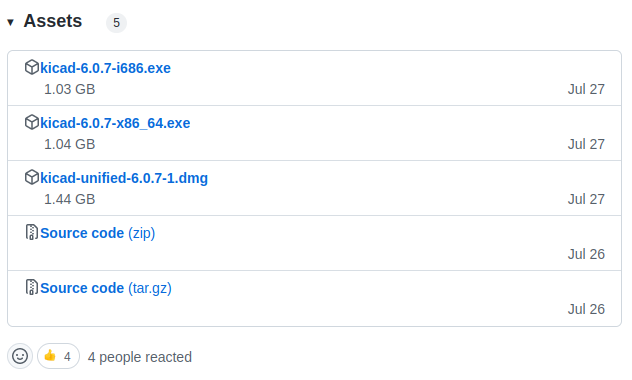
\includegraphics[width=0.75\textwidth]{images/installations/kicad_github}
		\caption{Download KiCAD}
	\end{figure}

	Ukuran berkas instalasi berkisar 1GB.\\

	\textbf{TIPS:} Penulis hanya merekomendasikan sumber instalasi dari URL Github di atas.
	Selain merupakan sumber resmi, juga Github menyediakan kecepatan download cukup tinggi.\\

	\textbf{TIPS:} Jika dibutuhkan versi 5 (seperti untuk Windows 7), dapat dikunjungi alamat berikut:\\
	\url{https://downloads.kicad.org/kicad/windows/explore/stable}\\

	Tutorial ini hanya akan menjelaskan KiCAD versi 6.

	\newpage
	\subsubsection{Proses Instalasi}

	Jalankan program installer yang telah di didownload. Klik \textit{Next}

	\begin{figure}[!ht]
		\centering
		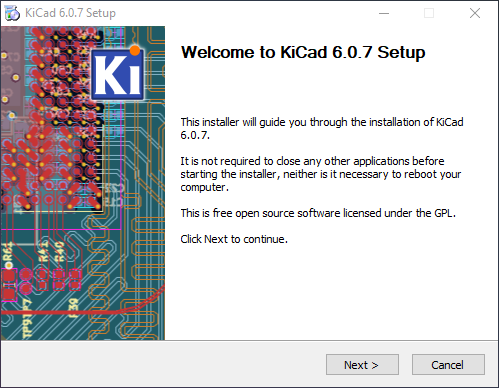
\includegraphics[width=0.7\textwidth]{images/installations/kicad_install_0}
		\caption{Memulai Instalasi KiCAD}
	\end{figure}

	Pilih paket apa saja yang ingin diinstal.
	Disini dapat di-\textit{unselect} paket Footprint 3D jika ada ingin menghemat 5GB instalasi.
	Lanjut klik \textit{Next}

	\begin{figure}[!ht]
		\centering
		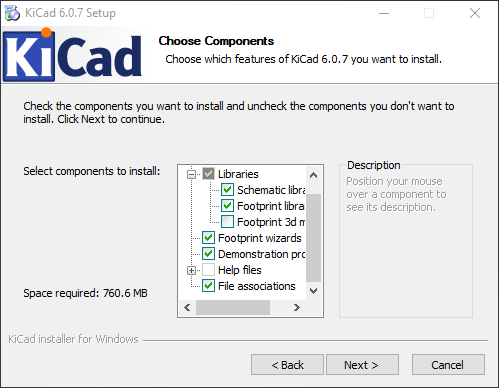
\includegraphics[width=0.7\textwidth]{images/installations/kicad_install_1}
		\caption{Pilih Paket}
	\end{figure}

	\newpage
	Tunggu proses instalasi hingga selesai

	\begin{figure}[!ht]
		\centering
		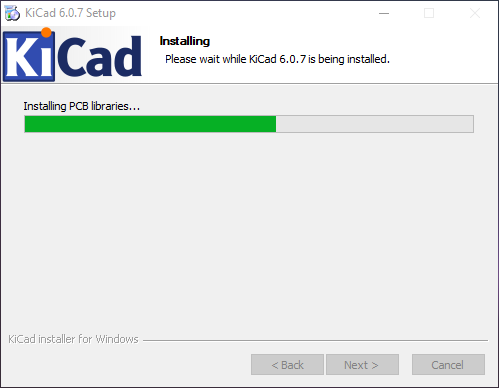
\includegraphics[width=0.7\textwidth]{images/installations/kicad_install_2}
		\caption{Proses Instalasi}
	\end{figure}

	Setelah instalasi selesai, dapat diklik \textit{Finish}.
	Tidak perlu install FreeCAD untuk saat ini.

	\begin{figure}[!ht]
		\centering
		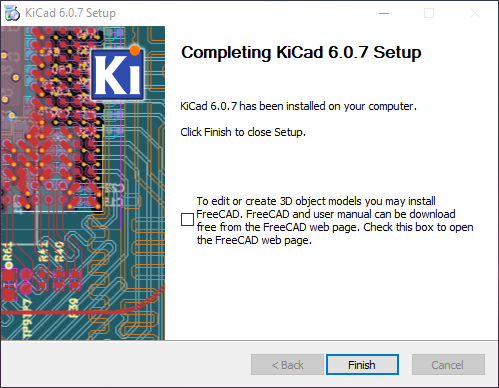
\includegraphics[width=0.7\textwidth]{images/installations/kicad_install_3}
		\caption{Instalasi Selesai}
	\end{figure}

	\newpage
	\subsection{MacOS}
	Nanti akan dilengkapi saat penulis cukup berduit untuk memiliki laptop Apple dan MacOS.

	\section{Memulai Program}

	Untuk memulai program KiCAD pada GNU/Linux, dapat digunakan perintah:
	\begin{lstlisting}
kicad
	\end{lstlisting}

	Atau dapat pula melalui menu sistem seperti pada sistem operasi Windows

	\begin{figure}[!ht]
		\centering
		\begin{subfigure}[t]{0.4\textwidth}
			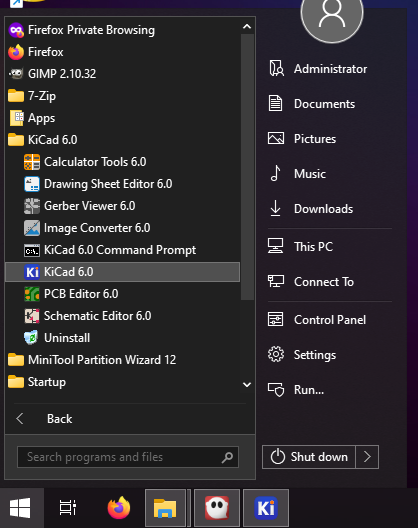
\includegraphics[width=\textwidth]{images/installations/kicad_menu_all}
			\caption{Windows 10}
		\end{subfigure}
		\begin{subfigure}[t]{0.4\textwidth}
			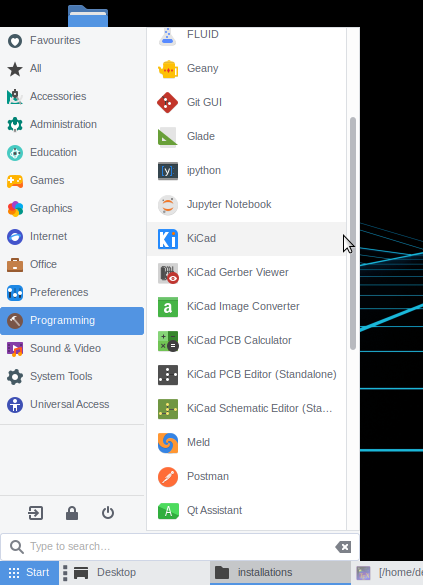
\includegraphics[width=\textwidth]{images/installations/kicad_menu_linux}
			\caption{Arch Linux}
		\end{subfigure}
		\caption{Memulai KiCAD via menu sistem operasi}
	\end{figure}

	Jika instalasi sukses, akan tampil pilihan migrasi pengaturan.
	Pilih default saja dan klik \textit{OK}.

	\begin{figure}[!ht]
		\centering
		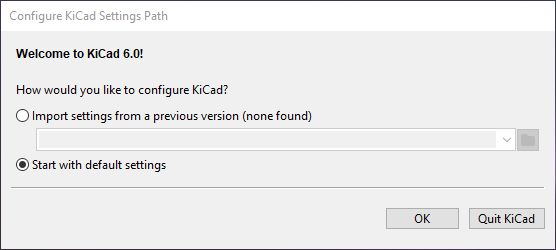
\includegraphics[width=0.7\textwidth]{images/installations/kicad_welcome}
		\caption{Migrasi Pengaturan}
	\end{figure}

	\newpage
	Tunggu beberapa saat, maka program utama KiCAD akan muncul.

	\begin{figure}[!ht]
		\centering
		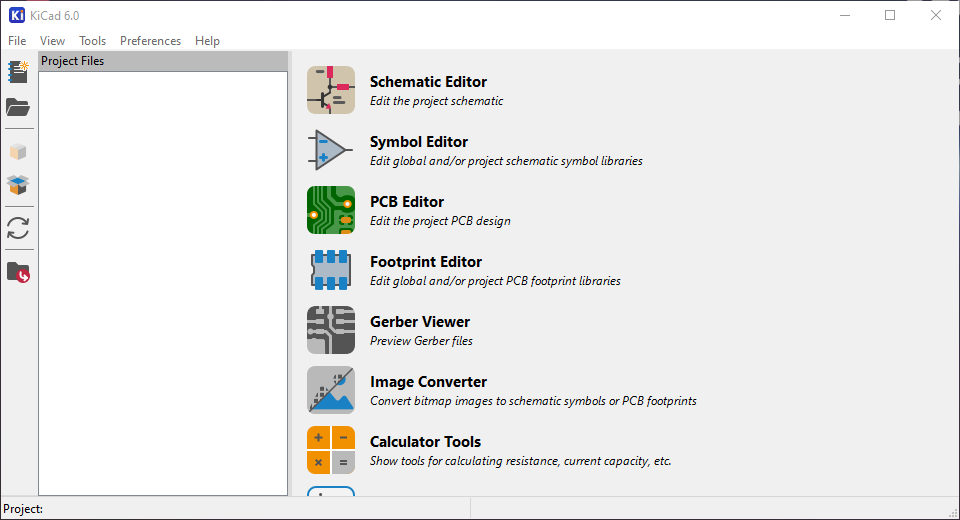
\includegraphics[width=\textwidth]{images/installations/kicad_first}
		\caption{Program Utama KiCAD}
	\end{figure}

	\textbf{PERINGATAN:} Jika saat menjalankan KiCAD muncul pesan OpenGL error seperti di bawah ini:

	\begin{figure}[!ht]
		\centering
		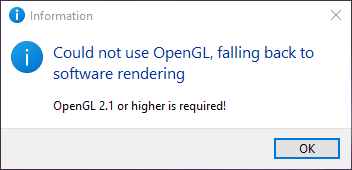
\includegraphics[width=0.7\textwidth]{images/installations/kicad_warn_noopengl}
		\caption{Peringatan OpenGL}
	\end{figure}

	Maka besar kemungkinan driver display atau VGA komputer masih menggunakan driver bawaan Windows.
	Silahkan update driver display komputer anda sesuai hardware yang terpasang.\\

	\begin{center}
		\textbf{Sampai disini, proses instalasi telah selesai.}
	\end{center}

	%%%%%%%%%%%%%%%%%%%%%%%%%%%%%%%%%%%%%%%%%%%%%%%%%%%%%%%%%%%%%%%%%

	\newpage
	\chapter{Dasar Konsep}

	\section{Program Utama}

	Berikut program utama KiCAD:

	\begin{figure}[!ht]
		\centering
		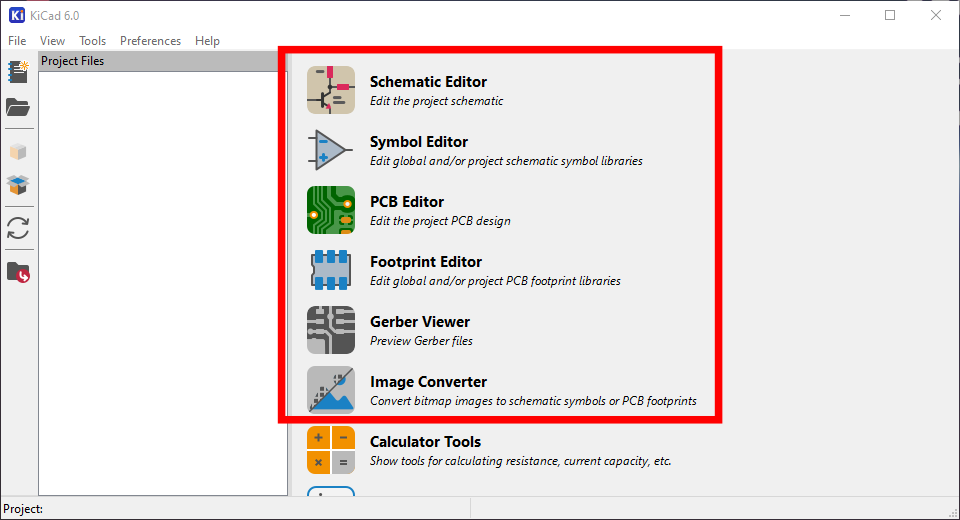
\includegraphics[width=\textwidth]{images/main/kicad_main}
		\caption{Program Utama KiCAD}
	\end{figure}

	Terdiri dari:
	\begin{itemize}
		\item \textbf{Schematic Editor}. Program menggambar skematik sirkuit.
		\item \textbf{Symbol Editor}. Program modifikasi atau membuat sendiri simbol komponen.
		\item \textbf{PCB Editor}. Program menggambar layout PCB.
		\item \textbf{Footprint Editor}. Program modifikasi atau membuat sendiri footprint (representasi aktual) komponen.
		\item \textbf{Gerber View}. Program menampilkan berkas-berkas Gerber
		\item \textbf{Image Converter}. Program mengkonversi gambar ke footprint
	\end{itemize}

	Mengingat ini adalah panduan dasar, maka Symbol Editor dan Footprint Editor tidak dibahas.

	\newpage
	\section{Workflow}

	\begin{figure}[!ht]
		\centering
		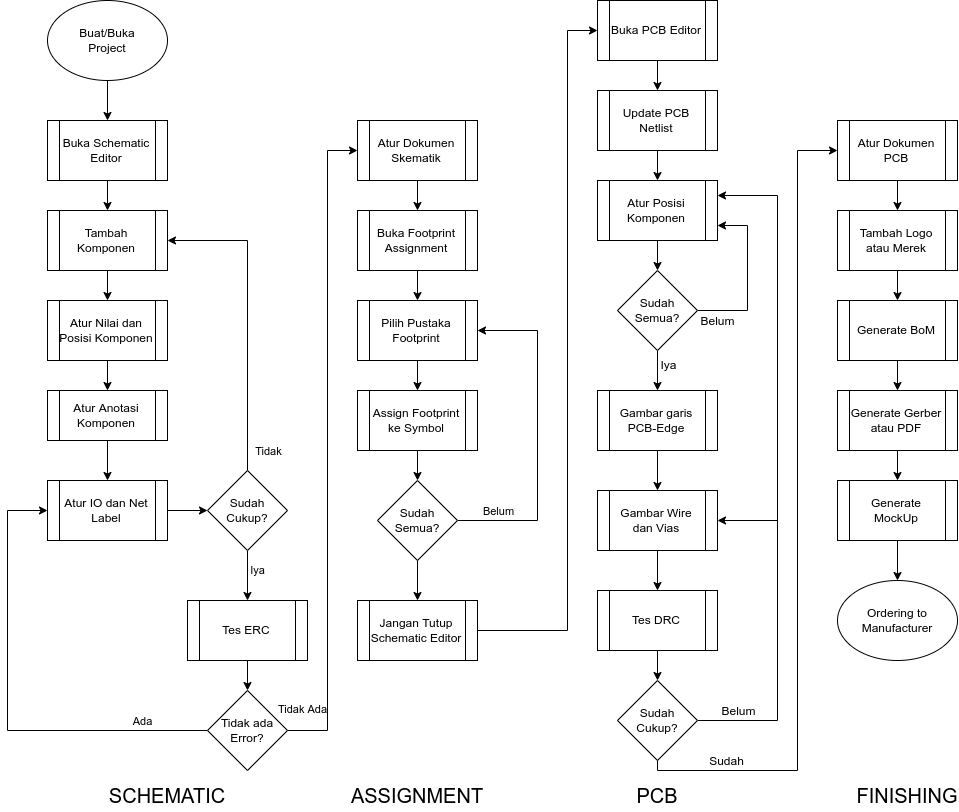
\includegraphics[width=0.9\textwidth]{images/main/kicad_workflow}
		\caption{Workflow Utama KiCAD}
	\end{figure}

	\textbf{TIPS:} Tidak perlu menghafal secara fix untuk proses diagram di atas, cukup dijadikan sebagai panduan umum.

	\section{Daftar Komponen}

	Untuk Daftar Komponen yang digunakan dalam tutorial kali ini, berikut tabelnya:\\

	\begin{table}[h!]
	\begin{center}
		\begin{tabular}{|l|l|l|l|l|l|}
		\toprule
		Parts & Example & Parts & Example & Parts & Example \\
		\midrule
		ESP32-WROOM & \href{https://www.tokopedia.com/akhishop/esp-32-esp-32s-esp-wroom-32-wifi-bluetooth-dual-core-chip}{Tokopedia} &
		Photoresistor & \href{https://www.tokopedia.com/ardushopid/sensor-cahaya-photoresistor-ldr-arduino}{Tokopedia} &
		LED 1206 & \href{https://www.tokopedia.com/alef/led-1206-smd-putih-white-lampu}{Tokopedia} \\
		\midrule
		Resistor 1206 & \href{https://www.tokopedia.com/isee/resistor-smd-1206-10kohm-10k-10-kilo-ohm-toleransi-1-tolerance-1}{Tokopedia} &
		Trimpot SMD & \href{https://www.tokopedia.com/digiware/vr-500k-ohm-singleturn-3314j-variable-resistor-trimpot-smd}{Tokopedia} &
		PC817 SMD & \href{https://www.tokopedia.com/putraniagabdg/pc817-smd-optocoupler-pc-817-sop-4pin-el817-pc817-1-high-quality}{Tokopedia} \\
		\bottomrule
		\end{tabular}
		\caption{Contoh Komponen}
	\end{center}
	\end{table}

	\newpage
	\section{Project Baru}

	Untuk membuat project kosong baru, klik icon \textit{Create New Blank Project} seperti digambar ini:

	\begin{figure}[!ht]
		\centering
		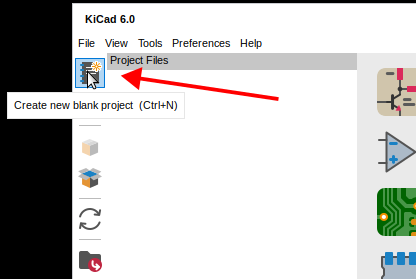
\includegraphics[width=0.4\textwidth]{images/main/kicad_new_0}
		\caption{Project Baru}
	\end{figure}

	Pilih folder dan beri nama project tersebut. Contoh disini adalah \textbf{esp32relay}.

	\begin{figure}[!ht]
		\centering
		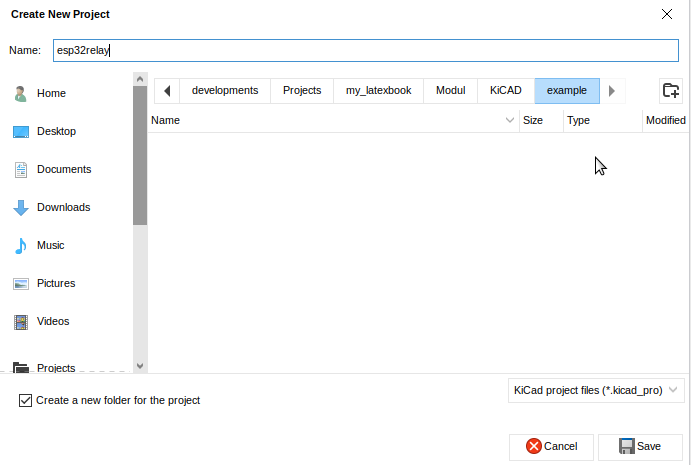
\includegraphics[width=0.5\textwidth]{images/main/kicad_new_1}
		\caption{Nama Project}
	\end{figure}

	Kemudian akan menghasilkan 3 berkas utama, yaitu \textbf{*.kicad\_pro} (berkas project),
	\textbf{*.kicad\_sch} (berkas skematik), dan \textbf{*.kicad\_pcb} (berkas PCB).

	\begin{figure}[!ht]
		\centering
		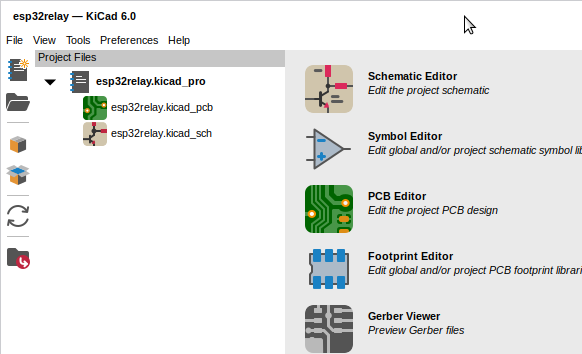
\includegraphics[width=0.6\textwidth]{images/main/kicad_new_2}
		\caption{Berkas Project}
	\end{figure}

	%%%%%%%%%%%%%%%%%%%%%%%%%%%%%%%%%%%%%%%%%%%%%%%%%%%%%%%%%%%%%%%%%

	\newpage
	\chapter{Skematik}
	Skematik adalah dokumen rancang sirkuit elektronik yang berisi simbol komponen beserta jaringan sinyal pinout atau catu daya.

	\section{Schematic Editor}

	Program Schematic Editor dapat dijalankan melalui program utama KiCAD:

	\begin{figure}[!ht]
		\centering
		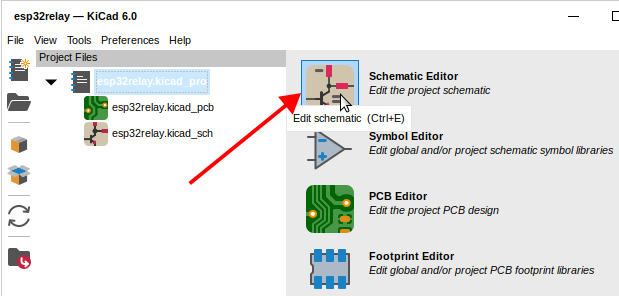
\includegraphics[width=0.6\textwidth]{images/sch/sch_0}
		\caption{Memanggil editor skematik}
	\end{figure}

	Jika baru pertama kali dijalankan akan ada konfirmasi pengaturan sumber pustaka symbol.
	Pilih saja yang direkomendasikan dan klik \textit{OK}.

	\begin{figure}[!ht]
		\centering
		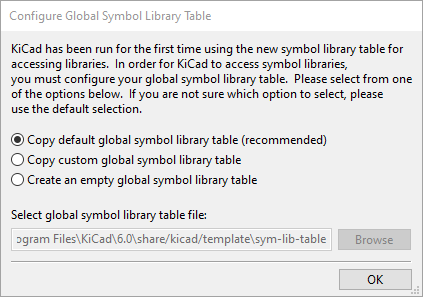
\includegraphics[width=0.5\textwidth]{images/installations/kicad_first_sch}
		\caption{Pilihan sumber pustaka}
	\end{figure}

	\newpage
	Berikut tampilan awal Schematic Editor
	\begin{figure}[!ht]
		\centering
		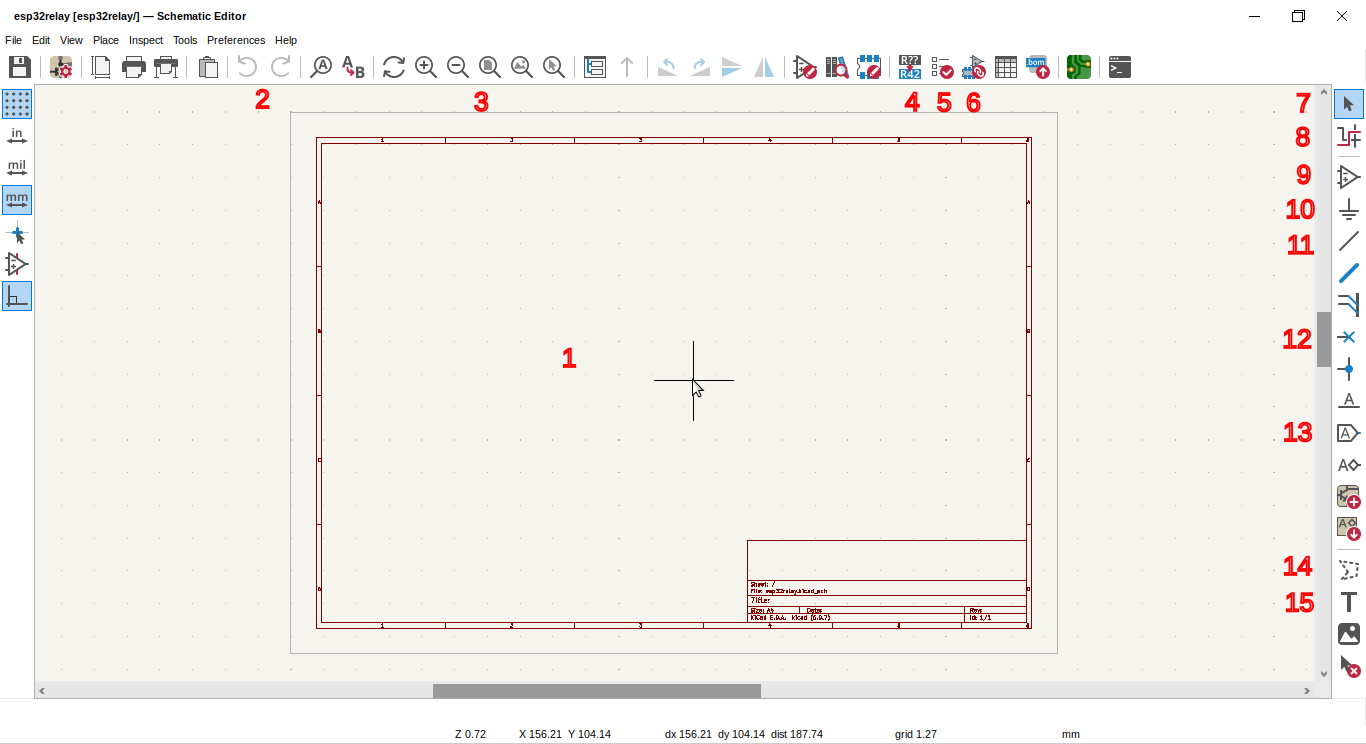
\includegraphics[width=\textwidth]{images/sch/sch_1}
		\caption{Schematic Editor}
	\end{figure}

	Penjelasan singkat tiap bagian:
	\begin{enumerate}[label=\textbf{\arabic*}.]
		\item Kanvas untuk menggambar skematik
		\item Toolbar perintah Undo-Redo
		\item Toolbar pengaturan tampilan skematik
		\item Toolbar perintah Anotasi komponen
		\item Toolbar perintah test ERC
		\item Toolbar perintah untuk Footprint Assignment
		\item Mode pointer default
		\item Mode tracking jalur baik di skematik maupun PCB
		\item Mode menambahkan komponen
		\item Mode menambahkan jaringan catu daya
		\item Mode menambahkan wiring
		\item Mode penanda Not-Connected
		\item Mode label sinyal
	\end{enumerate}

	\textbf{PERHATIAN:} Panduan selanjutnya akan menggunakan angka-angka di atas sebagai acuan.\\

	\textbf{TIPS:} Untuk memanipulasi objek di skematik maupun PCB, dapat melalui klik kanan objek yang ingin dimanipulasi.
	Sementara klik kanan pada area kosong dapat digunakan untuk menggeser kanvas.

	\newpage
	\section{Part ESP32}

	\subsubsection{Penempatan Komponen}

	Selanjutnya untuk menambahkan komponen, kita dapat klik menu \textit{Place -> Add Symbol}, atau klik \textbf{No:9}.
	Akan muncul dialog database komponen, cari dengan term \textbf{esp32}.

	Pilih komponen ESP32-WROOM-32, pada dialog akan tampil pratinjau symbol dan default footprint yang tersedia.
	\begin{figure}[!ht]
		\centering
		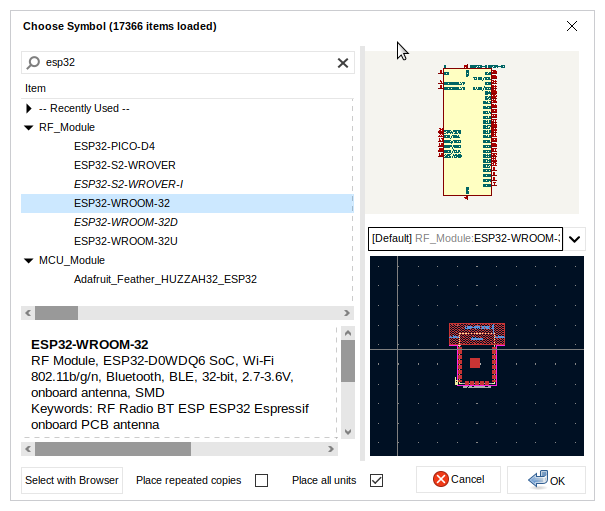
\includegraphics[width=0.6\textwidth]{images/sch/sch_2}
		\caption{Dialog Komponen}
	\end{figure}

	Untuk memulai penempatan komponen, klik \textit{OK}

	\begin{figure}[!ht]
		\centering
		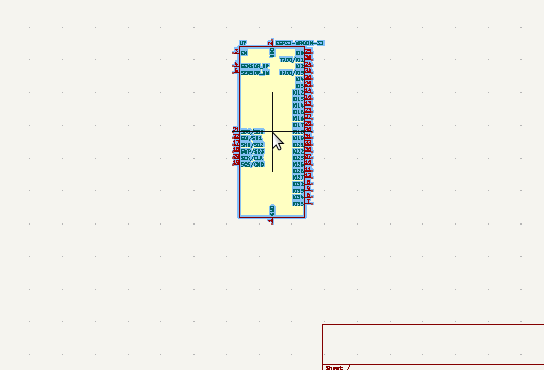
\includegraphics[width=0.6\textwidth]{images/sch/sch_3}
		\caption{Penempatan ESP32}
	\end{figure}

	Geser mouse ke tempat yang anda anggap cocok, tekan klik kiri untuk menempatkan.
	Anda juga dapat melakukan zoom-in dan zoom-out menggunakan roda mouse.

	Jika setelah menempatkan komponen kembali muncul dialog database komponen, silahkan tekan \textit{Cancel}.

	\newpage
	\subsubsection{Penambahan Sinyal}

	Selanjutnya kita melakukan penambahan jaringan sinyal ke komponen ESP32.
	Sebagai contoh pertama kita tambahkan sinyal TX0 (transmitter untuk UART).
	Klik \textit{Place -> Add Global Label} atau klik \textbf{No:13}.

	\begin{figure}[!ht]
		\centering
		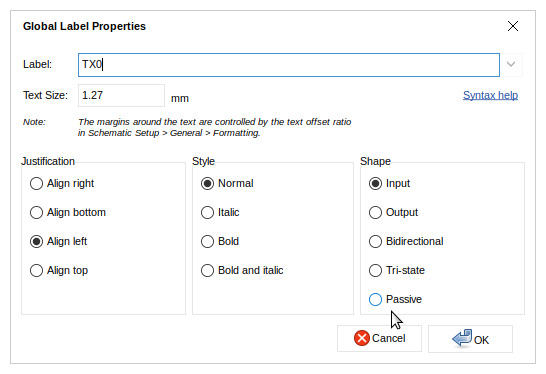
\includegraphics[width=0.5\textwidth]{images/sch/sch_4}
		\caption{Sinyal Properties}
	\end{figure}

	Isi nama sinyal dengan \textbf{TX0} dan klik \textit{OK}.
	Kemudian tempatkan label sinyal pada IO1 dengan pangkal-lingkar bertemu pangkal-lingkar seperti di bawah ini:

	\begin{figure}[!ht]
		\centering
		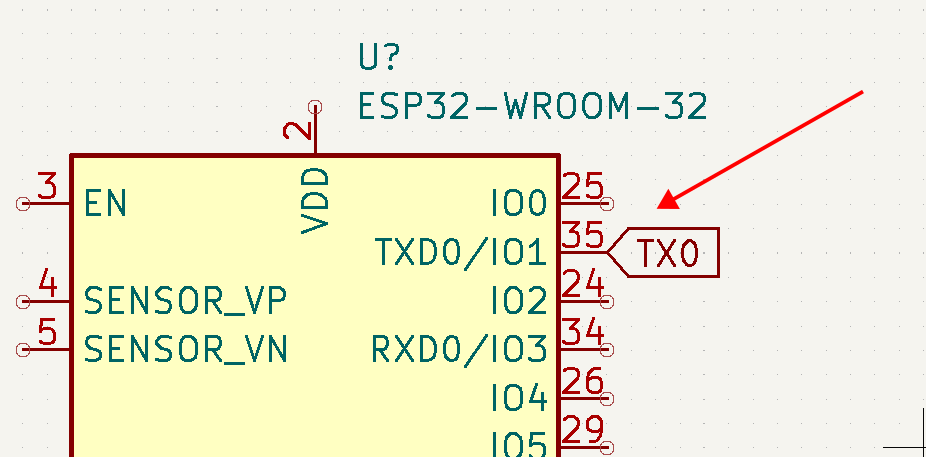
\includegraphics[width=0.5\textwidth]{images/sch/sch_5}
		\caption{Sinyal TX0}
	\end{figure}

	Kemudian dengan cara serupa, tempatkan sinyal \textbf{RX0} ke IO3

	\begin{figure}[!ht]
		\centering
		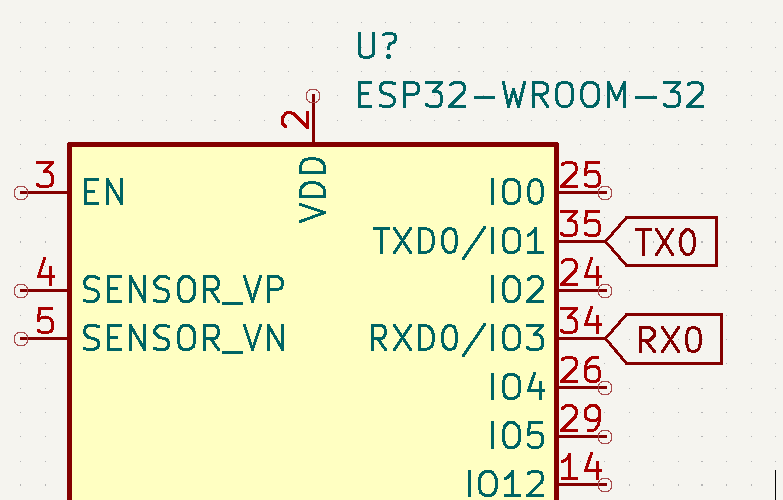
\includegraphics[width=0.5\textwidth]{images/sch/sch_6}
		\caption{Sinyal RX0}
	\end{figure}

	\newpage
	Lanjutkan penambahan sinyal mengikuti tabel berikut:

	\begin{table}[h!]
		\begin{center}
			\begin{tabular}{|l|l|l|l|l|l|}
				\toprule
				Sinyal & IO & Sinyal & IO & Sinyal & IO \\
				\midrule
				TX0 & IO1 & RX0 & IO3 & LED & IO2 \\
				FLASH & IO0 & RESET & EN & RELAY & IO18 \\
				ADC2\_CH4 & IO13 & ADC2\_CH6 & IO14 & - & - \\
				\bottomrule
			\end{tabular}
			\caption{ESP32 Sinyal IO}
		\end{center}
	\end{table}

	\begin{figure}[!ht]
		\centering
		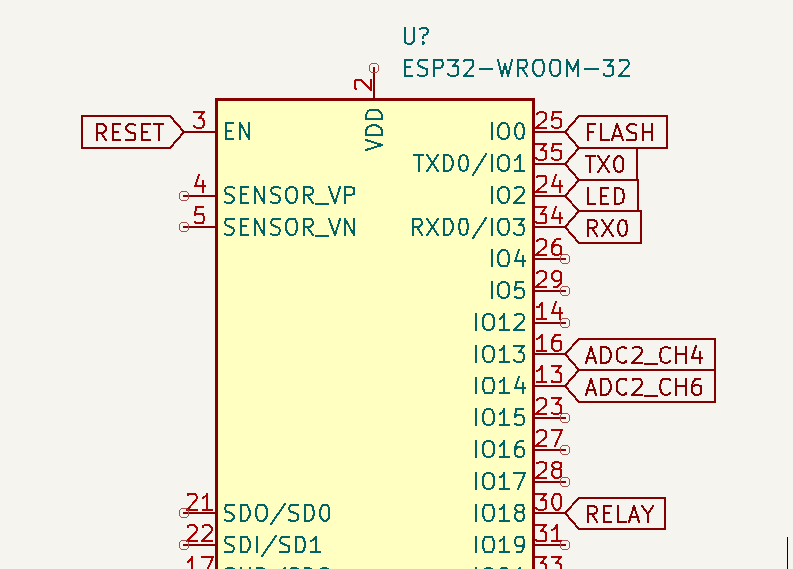
\includegraphics[width=0.5\textwidth]{images/sch/sch_7}
		\caption{Sinyal Utama}
	\end{figure}

	\textbf{TIPS:} Untuk manipulasi objek di skematik, selain menggunakan klik kanan, dapat pula menggunakan
	keyboard shortcut:
	\begin{itemize}
		\item \textbf{m}. Move atau memindahkan objek.

		\item \textbf{r}. Rotate atau memutar objek.

		\item \textbf{f}. Flip atau menukar orientasi objek.
	\end{itemize}

	Untuk objek \textit{Global Label}, memanipulasi tanpa menekan shortcut di atas akan mengubah posisi objek namun wiring tetap tersambung.

	\subsubsection{Penambahan Jalur Daya}

	Jalur daya akan ditambahkan disini adalah \textbf{VDD} (3.3v) dan acuan \textbf{GND} (0v).
	Klik menu \textit{Place -> Add Power} atau kli \textbf{No:10}.

	\begin{figure}[!ht]
		\centering
		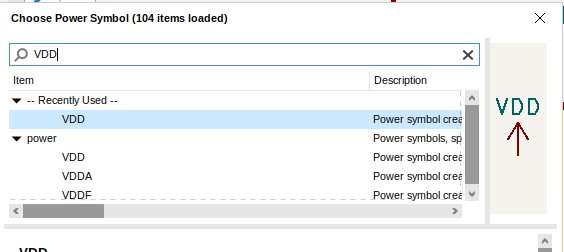
\includegraphics[width=0.4\textwidth]{images/sch/sch_8}
		\caption{Dialog Catu Daya}
	\end{figure}

	\textbf{TIPS:} Secara mendasar, jalur catu daya dapat diperlakukan sebagaimana layaknya komponen

	\begin{figure}[!ht]
		\centering
		\begin{subfigure}[t]{0.1\textwidth}
			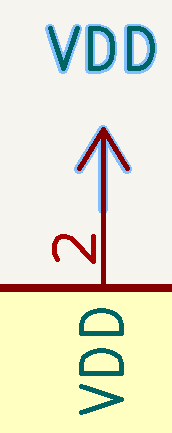
\includegraphics[width=\textwidth]{images/sch/sch_vdd}
			\caption{VDD}
		\end{subfigure}
		\begin{subfigure}[t]{0.1\textwidth}
			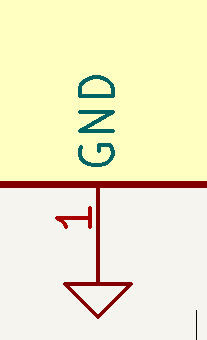
\includegraphics[width=\textwidth]{images/sch/sch_gnd}
			\caption{GND}
		\end{subfigure}
		\caption{Jalur catu daya}
	\end{figure}

	\subsubsection{Resistor Pull Down}

	Pada ESP32, jalur IO5 dan IO12 perlu ditarik ke level GND untuk memastikan booting chip.
	Untuk itu perlu ditambahkan resistor 0 ohm yang menghubungkan IO tersebut ke GND.

	Untuk menambahkan Resistor, kembali ke menu \textit{Place -> Add Symbol} atau klik \textbf{No:9}.
	Masukkan \textbf{R} ke kolom search.

	\begin{figure}[!ht]
		\centering
		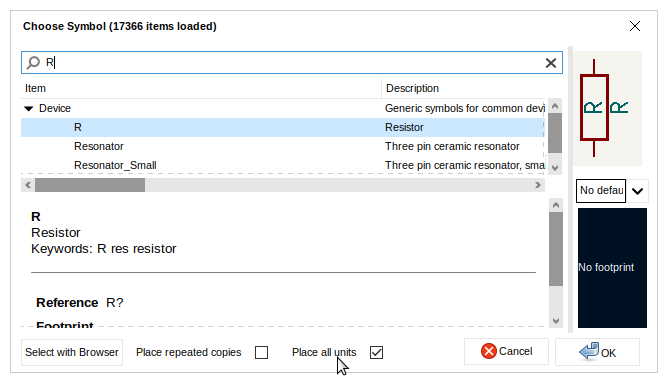
\includegraphics[width=0.55\textwidth]{images/sch/sch_9}
		\caption{Resistor}
	\end{figure}

	\textbf{PERHATIAN:} Resistor hanya memiliki default symbol, namun untuk footprint akan
	ditentukan nanti saat Assignment.\\

	Tempatkan Resistor dekat IO5
	\begin{figure}[!ht]
		\centering
		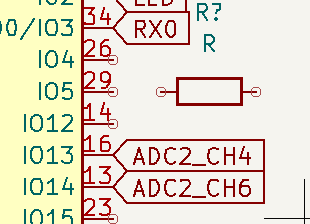
\includegraphics[width=0.4\textwidth]{images/sch/sch_10}
		\caption{Resistor IO5}
	\end{figure}

	Untuk memodifikasi nilai, double-klik huruf R yang tidak ada simbol (?) di dekatnya.
	\begin{figure}[!ht]
		\centering
		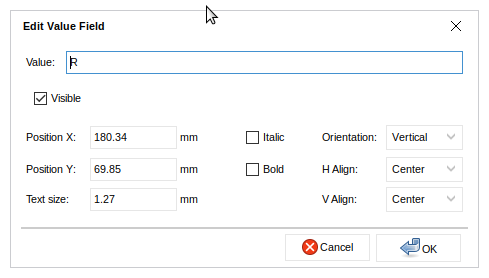
\includegraphics[width=0.55\textwidth]{images/sch/sch_11}
		\caption{Ganti Nilai}
	\end{figure}

	Ganti huruf \textbf{R} menjadi angka \textbf{0}. Kemudian klik \textit{OK}.

	\begin{figure}[!ht]
		\centering
		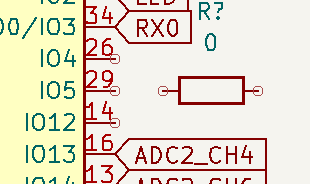
\includegraphics[width=0.55\textwidth]{images/sch/sch_12}
		\caption{Resistor 0 untuk IO5}
	\end{figure}

	Duplikat resistor tersebut dengan klik kanan dan klik \textit{Duplicate}
	atau langsung tekan CTRL+d di keyboard.
	Taruh komponen duplikat dekat IO12.\\

	\textbf{TIPS:} Anda dapat pula menggeser nilai dan nama komponen agar terlihat lebih jelas.

	\begin{figure}[!ht]
		\centering
		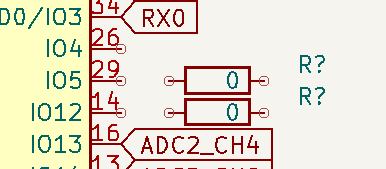
\includegraphics[width=0.55\textwidth]{images/sch/sch_13}
		\caption{Resistor 0 untuk booting}
	\end{figure}

	Selanjutnya ambil satu GND dan letakkan dekat kedua komponen tersebut.

	\newpage
	Kemudian karena komponen berdekatan, dapat dipilih menghubungkan pangkal-lingkar komponen
	menggunakan wiring.
	Klik menu \textit{Place -> Add Wire} atau klik \textbf{No:11}.\\

	Taruh pointer mouse ke salah satu pangkal-lingkar, klik kiri,
	kemudian geser ke pangkal-lingkar lain yang akan dihubungkan, kemudian klik kiri sekali lagi.\\

	Hubungkan wire hingga seperti ini:

	\begin{figure}[!ht]
		\centering
		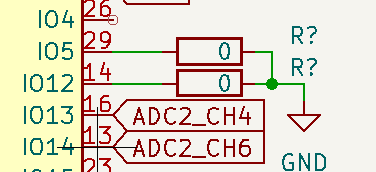
\includegraphics[width=0.5\textwidth]{images/sch/sch_14}
		\caption{Wire untuk untuk booting}
	\end{figure}

	\subsubsection{Menambahkan Anotasi}

	Proses Anotasi adalah mengubah simbol (?) menjadi angka yang dapat menjadi index pembeda antara
	satu komponen dengan komponen lain yang sejenis.
	Untuk melakukan Anotasi, klik menu \textit{Tools -> Annotate Schematic} atau klik \textbf{No:4}.
	Kemudian klik \textit{Annotate} dan \textit{Close} saat selesai.

	\begin{figure}[!ht]
		\centering
		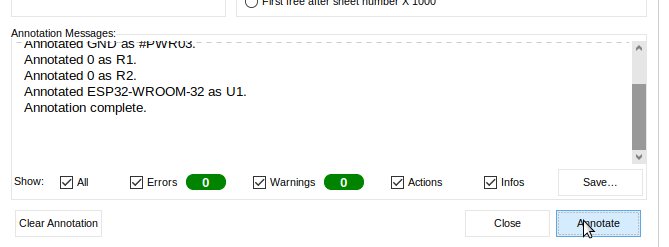
\includegraphics[width=0.6\textwidth]{images/sch/sch_15}
		\caption{Dialog Annotasi}
	\end{figure}

	Simbol (?) disebelah nama tiap komponen yang telah teranotasi akan tergantikan dengan angka.

	\begin{figure}[!ht]
		\centering
		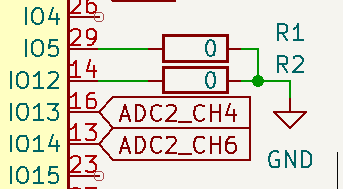
\includegraphics[width=0.5\textwidth]{images/sch/sch_16}
		\caption{Komponen telah teranotasi}
	\end{figure}

	\textbf{TIPS:} Jangan lupa simpan pekerjaan dengan klik menu \textit{File -> Save} atau tekan CTRL+s di keyboard.

\end{document}